\section{基本采样算法}
本节中,我们研究从一个给定的概率分布中生成随机样本的一些简单的方法。
\subsection*{标准概率分布}
首先,我们考虑如何从简单的非均匀分布中生成随机数,假定我们已经有了一个均匀分布的随机数的来源。假设$z$在区间$(0,1)$上均匀分布,我们使用某个函数$f(\cdot)$对$z$的值进行变换,即$y=f(z)$。$y$上的概率分布为
\begin{equation}
\label{suiji}
	p(y)=p(z)\bigg|\frac{\mathrm{d}z}{\mathrm{d}y}\bigg|
\end{equation}
其中,在这种情况下,$p(z)=1$。我们的目标是选择一个函数$f(z)$使得产生出的$y$值具有某种所需的具体的分布形式$p(y)$,对公式$\ref{suiji}$进行积分,我们有
\begin{equation}
	z=h(y)\equiv \int _{-\infty}^{y}p(\hat{y})d\hat{y}
\end{equation}
它是$p(y)$的不定积分,因此$y=h^{-1}(z)$,因此我们必须使用一个函数来对这个均匀分布的随机数进行变换,这个函数是所求的概率分布的不定积分的反函数,如图所示
\begin{center}
	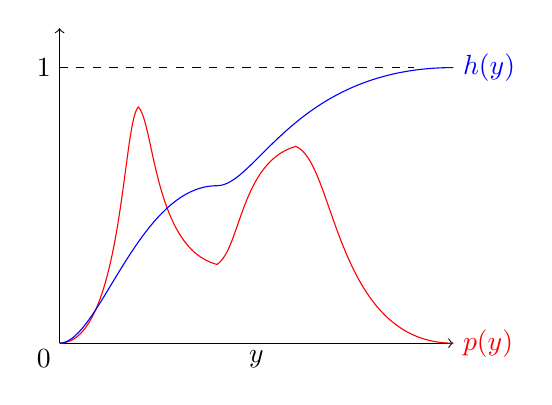
\begin{tikzpicture}
		\draw[->] (0,0) -- (5,0) node at (-0.2,3.5) {$1$};
		\draw[->] (0,0) -- (0,4) node at (-0.2,-0.2){$0$};
		\draw[dashed] (0,3.5) -- (4.5,3.5) node at (2.5,-0.2) {$y$};
		
		\draw[red]  
		(0,0) .. controls (0.8,0) and (0.8,2.8)  ..  (1,3) .. controls (1.2,2.8) and (1.2,1.2) .. (2,1) .. controls (2.3,1.2) and (2.3,2.3) .. (3,2.5) .. controls (3.5,2.3) and (3.5,0) .. (5,0) node[right] {$p(y)$};
		\draw[blue] (0,0) .. controls (0.5,0) and (1,2) .. (2,2) .. controls (2.5,2) and (3,3.5) ..(5,3.5) node[right] {$h(y)$};

	\end{tikzpicture}
\end{center}

考虑指数分布(exponential distribution)
\begin{equation}
	p(y)=\lambda \exp (-\lambda y)
\end{equation}
其中$0\leqslant y \leqslant \infty$。在这种情况下
\begin{equation}
	h(y)=\int_0^y f(y)dy=1-\exp (-\lambda y)
\end{equation}
从而,如果我们将均匀分布的变量$z$使用$y=-\lambda^{-1}\ln (1-z)$进行变换,那么$y$就会服从指数分布。
\begin{equation}
\begin{aligned}
	z&=h(y)=1-\exp (-\lambda y)\\
	y&=h^{-1}(z)\\
	 &\Rightarrow \exp(-\lambda y) = 1-z\\
	 &\Rightarrow -\lambda y = \ln (1-z)\\
	 &\Rightarrow y=-\frac{1}{\lambda}\ln (1-z)
\end{aligned}
\end{equation}

另一种可以应用变换方法的概率分布是柯西分布
\begin{equation}
	p(y)=\frac{1}{\pi}\frac{1}{1+y^2}
\end{equation}
这种情况下,不定积分的反函数可以用$\tan$函数表示。

对于多个变量情形的推广是很容易的,涉及到变量变化的Jacobian行列式,即
\begin{equation}
	p(y_1,\dots,y_M)=p(z_1,\dots,z_M)\bigg| \frac{\partial (z_1,\dots,z_M)}{\partial (y_1,\dots,y_M)}\bigg| 
\end{equation}

作为变换方法的最后一个例子,我们考虑Box-Muller方法,用于生成高斯概率分布的样本。首先我们生成一对均匀分布的随机变量$z_1,z_2\in (-1,1)$,我们可以这样生成:对$(0,1)$上的均匀分布的变量使用$z\to 2z -1$的方式进行变换。接下来,我们丢弃那些不满足$z_1^2+z_2^2\leqslant 1$的点对。这产生出单位圆内部的一个均匀分布,且$p(z_1,z_2)=\frac{1}{\pi}$。然后,对于每对$z_1,z_2$,我们计算 
\begin{flalign}
	y_1&=z_1\left(\frac{-2\ln r^2}{r^2} \right)^{\frac{1}{2}}\\
	y_2&=z_2\left(\frac{-2\ln r^2}{r^2} \right)^{\frac{1}{2}}
\end{flalign}
其中$r^2=z_1^2+z_2^2$。这样,$y_1$和$y_2$的联合概率分布为
\begin{equation}
	\begin{aligned}
		p(y_1,y_2)&=p(z_1,z_2)\bigg|\frac{\partial (z_1,z_2)}{\partial (y_1,y_2)} \bigg|\\
		&=\left[\frac{1}{\sqrt{2\pi}}\exp \left(\frac{-y_1^2}{2} \right) \right]\left[\frac{1}{\sqrt{2\pi}}\exp \left(\frac{-y_1^2}{2}\right) \right]
	\end{aligned}
\end{equation}
因此$y_1$和$y_2$是独立的,有每个都服从高斯分布,均值为零,方差为1。

\textbf{推导过程:}(Box-Muller变换原理)
\begin{enumerate}
	\item 目标
	\begin{equation}
	\begin{aligned}
		p(y_1,y_2)&=\left[\frac{1}{\sqrt{2\pi}}\exp \left(\frac{-y_1^2}{2} \right) \right]\left[\frac{1}{\sqrt{2\pi}}\exp \left(\frac{-y_1^2}{2}\right) \right]\\
		&=\frac{1}{2\pi}\exp \left(-\frac{y_1^2+y_2^2}{2} \right)
	\end{aligned}
	\end{equation}
	做极坐标变换,则$y_1=R\cos \theta,y_2=R\sin \theta$,则有
	\begin{equation}
		\frac{1}{2\pi}\exp \left(-\frac{y_1^2+y_2^2}{2} \right)=\frac{1}{2\pi}\exp \left(-\frac{R^2}{2} \right)
	\end{equation}
	可以看到这个结果可以看成是两个概率分布的密度函数的乘积,其中一个可以看成是$[0,2\pi]$上均匀分布,将其转换为标准均匀分布则有$\theta \sim U(0,2\pi)=2\pi z_1$,因为($z_1,z_2\sim U(0,1)$)。
	\item 求$h(y_1,y_2)$
	\begin{equation}
		\begin{aligned}
			z&=P(R\leqslant r)\\
			 &=\int_0^{2\pi} d\theta\int_0^r \frac{1}{2\pi}\exp \left(-\frac{\rho^2}{2} \right)\rho d\rho\\
			 &=-\exp\left(\frac{-\rho^2}{2}\right)\bigg|_0^r \\
			 &=-\exp \left(-\frac{r^2}{2}\right)+1
		\end{aligned}
	\end{equation}
	其中$r^2=z_1^2+z_2^2$。
	\item 求$y1,y2$
	\begin{equation}
		\begin{aligned}
			R&=h^{-1}(z)\\
			&=\sqrt{-2\ln (1-z)}
		\end{aligned}
	\end{equation}
	这里是二维联合分布,因此
	\begin{equation}
		\begin{aligned}
			y_1&=R\cos \theta = \frac{z_1}{r} \sqrt{-2\ln (r^2)}\\
			y_2&=R\sin \theta = \frac{z_2}{r} \sqrt{-2\ln (r^2)}
		\end{aligned}
	\end{equation}
\end{enumerate}

显然,变换方法依赖于它能够进行计算所需的概率分布,并且能够求所需的概率分布的不定积分的反函数。这样的计算只对于一些非常有限的简单的概率分布可行,因此我们必须寻找一些更加一般的方法。这里,我们考虑两种方法,即拒绝采样(rejection sampling)和重要采样(importance sampling)。虽然这些方法主要限制在单变量概率分布,因此无法直接应用于多维的复杂问题,但是这些方法确定是更一般的方法的重要成分。
\subsection*{拒绝采样}
拒绝采样框架使得我们能够在满足某些限制条件的情况下,从相对复杂的概率分布中采样。首先,我们考虑单变量分布,然后接下来讨论对于多维情形的推广。

假设我们希望从$p(\boldsymbol{z})$中采样,这个概率分布不是我们目前为止讨论过的简单的标准的概率分布中的一个,从而直接从$p(\boldsymbol{z})$中采样是很困难的。此外,我们假设我们能够很容易地计算对于任意给定的$\boldsymbol{z}$值的$p(\boldsymbol{z})$(不考虑归一化常数$Z$),即
\begin{equation}
	p(z)=\frac{1}{Z_p}\tilde{p}(z)
\end{equation}
其中$\tilde{p}(z)$可以很容易地计算,但是$Z_p$未知。

为了应用拒绝采样方法,我们需要一些简单的概率分布$q(z)$,有时被称为提议分布(proposal distribution),并且我们已经可以从提议分布中进行采样。接下来,我们引入一个常数k,它的值的选择满足下面的性质:对所有的z值,都有$kq(z)\geqslant \tilde{p}(z)$。函数$kq(z)$被称为比较函数。

拒绝采样器的每个步骤涉及到生成两个随机数。首先,我们从概率分布$q(z)$中生成一个数$z_0$。接下来,我们在区间$[0,kq(z)]$上的均匀分布中生成一个数$u_0$。这对随机数在函数$kq(z)$的曲线下方是均匀分布。最后,如果$u_0>\tilde{p}(z_0)$,那么样本被拒绝,否则$u_0$被保留。因此对应的$z$值服从概率分布$p(z)$,正如我们所需的那样。
\begin{center}
	\begin{tikzpicture}
		\filldraw[gray!50,line width=2] (-3,1) .. controls (-1,1) and (0,4).. (1,4) .. controls (2,4) and (3,1).. (5,1);
		\draw[pattern=north west lines,gray!50] (-3,0.1) rectangle (5,1);
		
		\filldraw[line width=2,draw=red,white] (-1.5,0.1) .. controls (-1,0.1) and (-0.7,2).. (0,2) .. controls (0.3,2) and (0.7,1).. (1,1).. controls (1.3,1) and (1.5,3).. (2,3) .. controls (2.5,3) and (2.5,0.1).. (4,0.1);
		
		\draw[->] (-3,0) -- (5,0) node[below] at (0,0){$z_0$};
		\draw[->] (0,0) -- (0,4);
		
		\node[fill,draw,circle,inner sep=0.5mm,black,label=left:$u_0$] at (0,1) {};
		\node[fill,draw,circle,inner sep=0.5mm,black,label=left:$kq(z_0)$] at (0,3.3) {};
		\node[label=left:$\tilde{p}(z)$] at (3,1) {};
		\node[black,label=left:$kq(z)$] at (3,4) {};
	\end{tikzpicture}
\end{center}
$z$的原始值从概率分布$q(z)$中生成,这些样本之后被接受的概率为$\frac{\tilde{p}(z)}{kq(z)}$,因此一个样本会被接受的概率为
\begin{equation}
	\begin{aligned}
		p(\text{接受})&=\int \left\{\frac{\tilde{p}(z)}{kq(z)} \right\}q(z)dz\\
		&=\frac{1}{k}\int \tilde{p}(z)dz
	\end{aligned}
\end{equation}
因此,被这种方法拒绝的点的比例依赖于曲线$kq(z)$下方的未归一化概率分布$\tilde{p}(z)$的面积的比例。于是,我们看到,常数k应该尽量小,同时满足下面的限制条件:$kq(z)$一定处处不小于$\tilde{p}(z)$。
\subsection*{可调节的拒绝采样}
在许多我们希望应用拒绝采样的情形中,确定概率分布$q(z)$的一个合适的解析形式是很困难的。另一种确定其函数形式的方法是基于概率分布$p(z)$的值直接构建函数形式。
\subsection*{重要采样}
\subsection*{采样-重要性-重采样}
\subsection*{采样与EM算法}
